\section{Background on FASTER}
\label{sec:fasterkv}

Shadowfax is built over the \faster single-node KVS, which it relies on for
hash indexing and record storage.
%
Here, we describe some key aspects of \faster, since Shadowfax's design
integrates with it and builds on its mechanisms.
%
More details about \faster itself can be found elsewhere~\cite{faster,cpr}.
%
Specifically, Shadowfax extends \faster's asynchronous
cuts, which help avoid coordination, and its \hlog, which transparently
spans DRAM and SSD.

\begin{figure}[t]
\centering
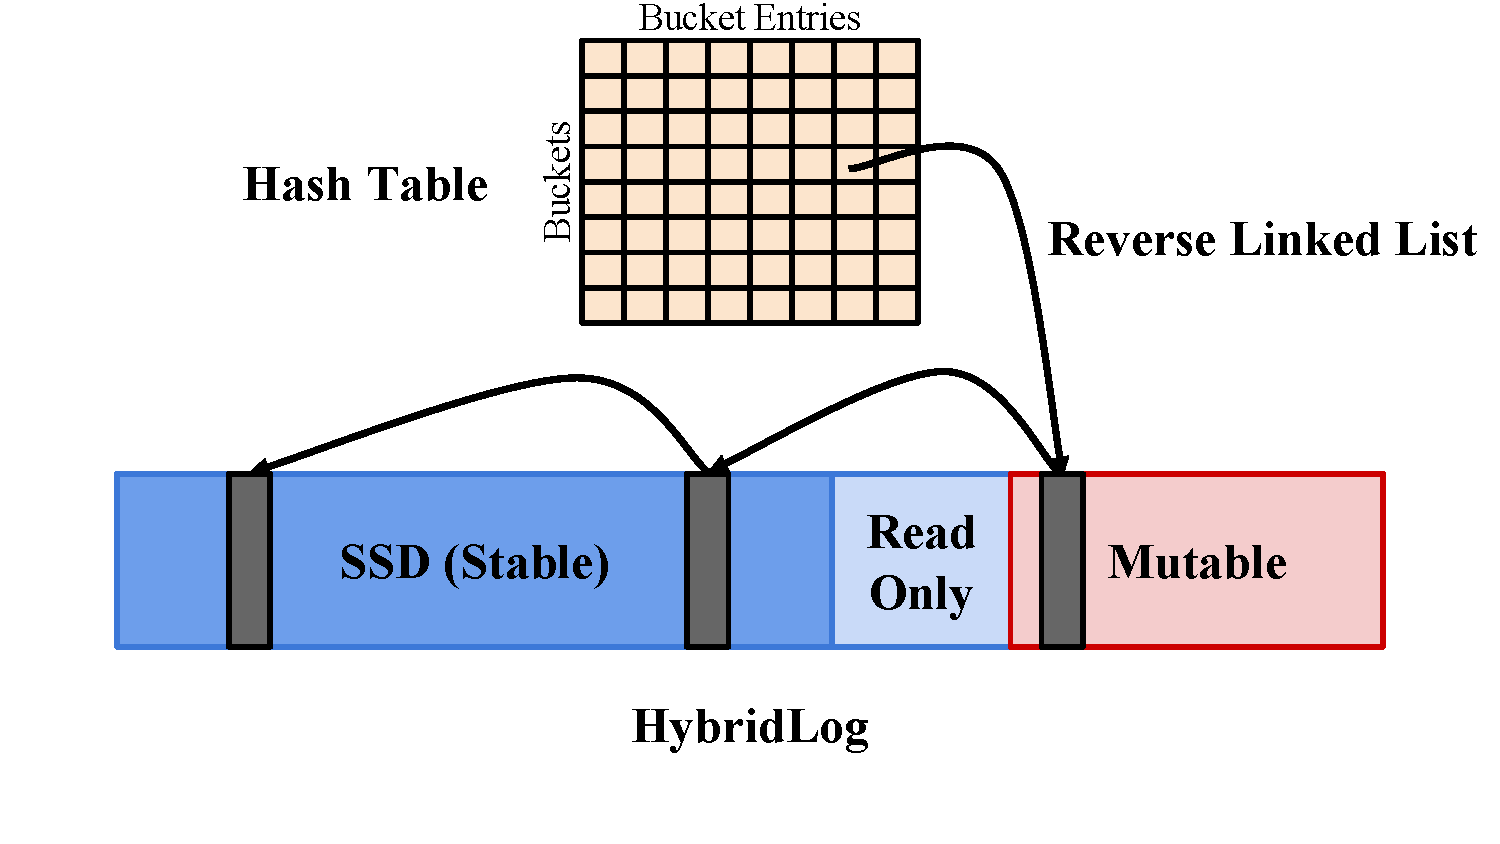
\includegraphics[width=\columnwidth]{figures/hybrid-log.pdf}
\vspace{-5ex}
\caption{\faster's \hlog allocator spans memory and local SSD.
    The portion in memory contains a mutable region that acts as a
    cache and a read-only region.
    \faster's hash table points to a reverse linked list of
    records on the \hlog.}
\label{fig:hlog}
\end{figure}


In most ways, \faster works like most durable hash table libraries.
%
It includes a lock-free hash table divided into cacheline-sized buckets
(Figure~\ref{fig:hlog}).
%
Each 8~byte bucket entry contains a pointer to a record whose key hashes to
that bucket.
%
Each record points to another record, forming a linked list of records with
common significant key hash bits.
%
Each bucket entry contains additional bits from the associated records' key
hash, increasing hashing resolution and disambiguating what records the bucket
entry points to without extra cache misses and without full key comparisons.
%
Each record pointed to by the hash table is stored in the \hlog.

\faster clients can use it like any other library, but a common pattern is to
pin one client application thread per CPU core to eliminate scheduler overheads.
%
Each client thread calls read or read-modify-write operations on keys in
\faster.
%
\faster's cache-conscious design and lock-freedom are key in its ability to
perform more than 100~Mops/s on a single multicore machine.
%
%Shadowfax uses \faster with a similar threading scheme described later.


\subsection{HybridLog Allocator}
\label{sec:hlog}

\faster allocates and stores all records in its \hlog, which spans memory and
SSD (Figure~\ref{fig:hlog}).
%
The \hlog combines in-place updates (for records in memory) and log-structured
organization (for records on SSD), and provides lock-free access to records.

The portion of the \hlog's address space on SSD forms the stable
region.
%
It contains cold records that have not been recently updated.
%
The portion in memory is composed of two regions: a (larger) mutable region and a
(smaller) read-only region.
%
Records in the mutable region can be modified in-place with appropriate
synchronization that is chosen by the application using \faster (for example, atomic
operations, locks, or validation).
%
This region acts as a cache for recently updated records and avoids expensive
per-update allocations.

The read-only region mostly contains records that are being asynchronously
written to SSD.
%
These records cannot be updated in place, since they must remain stable during I/O.
%
The read-only region represents records that are becoming cold, and it acts as
a second-chance cache.
%
\faster uses a read-copy-update to modify records in this region: the updated
record version is appended to the mutable region, and the hash table is updated to
point to it.
%
This helps provide good cache hit rates without fine-grained metadata.

Each record entry in \faster's hash table points to a reverse linked list of
records on the \hlog, allowing it to maintain a compact hash table for
\emph{larger-than-memory} datasets that span storage media.
%
Note, that a consequence of this is that hash table lookups in \faster may need
to traverse chains of records that span from memory onto SSD.
%
Section~\ref{sec:design:indirection} describes how Shadowfax extends \hlog so
that it also spans shared cloud storage and how this accelerates the completion
of scale out and data migration.



\subsection{Asynchronous Cuts}
\label{sec:epochs}

Lock-freedom makes \faster fast, but it creates challenges for synchronization
and memory safety.
%
Updated versions of records may be installed in its hash table, even as old
versions of that record are still being read by other threads.
%
This is a common problem in all lock-free, RCU-like schemes~\cite{rcu}.
%
To solve this, \faster uses an epoch-based memory-protection scheme~\cite{epochs}.
%
All threads calling into \faster are registered with an epoch manager that
tracks when threads begin and end access to \faster's internal structures.
%
When a page is evicted to SSD, the epoch-based scheme ensures that the memory
is not reused while any thread could still be accessing it.
%
The full details of this scheme are beyond the scope of this paper.

Critically, this epoch-based scheme also plays a key role in coordinating
information across threads lazily without inducing stalls.
%
During complex, process-wide events (such as page eviction and checkpointing), threads lazily
coordinate by registering callback actions that are eventually executed once each
thread synchronizes some local state with an updated
process-global value.
%
The same mechanism can also be used to trigger a function only once all threads
are guaranteed to have updated their local state from some process-global state.
%
In effect, this allows trigger actions that are guaranteed to
take effect only after all threads agree on and have each locally
observed some transition in process-global state.
%
This can be used to create a process-wide \emph{asynchronous cut}, where
events such as process state transitions are realized asynchronously and lazily
over a set of independent thread-local state transitions.

For instance, consider the read-offset address that demarcates read-only records from mutable
records on the \hlog (Section~\ref{sec:hlog}). When this address is updated, each thread may
notice the update at different points in time, depending on when they refresh their epoch.
Eventually, when all threads have observed the update, the records between the old and new
read-offsets have become read-only, and a function is triggered to write the pages to disk. Using the same
mechanism, addresses for which threads do not yet agree on the mutability status can be handled efficiently.
Figure~\ref{fig:cut} shows this process in action.

\begin{figure}[t]
\centering
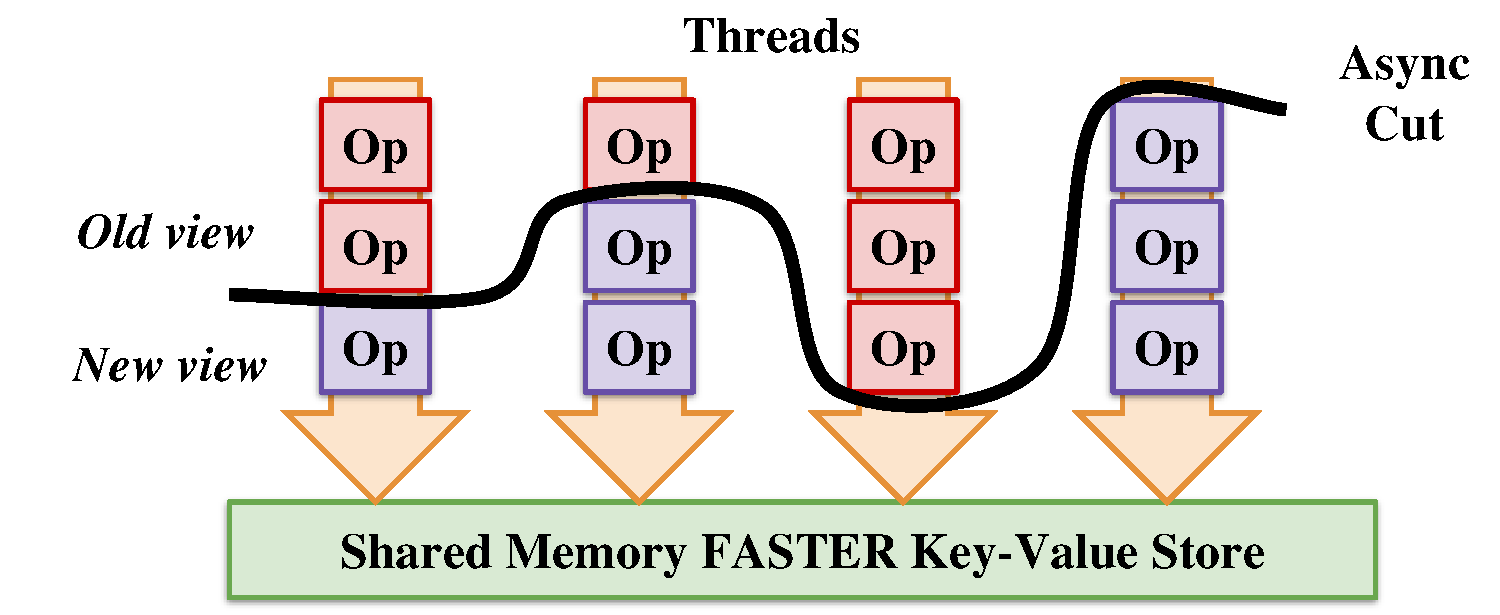
\includegraphics[width=\columnwidth]{figures/global-cut.pdf}
\caption{View changes of shared state in \faster take place over
    an asynchronous cut using epochs. Process-global state is updated first; when
    every thread has observed the update, a postchange function is triggered.}
\label{fig:cut}
\end{figure}


\iffalse
\faster's checkpointing protocol serves as a great example of this~\cite{cpr}.
%
It first moves all threads from a system checkpoint version $v$ to a
new checkpoint version $v+1$, and then it captures and persists records in
version $v$.
%
As threads process operations, they stamp each new record version they create
with their local checkpoint version number.
%
The boundary between the two checkpoint versions $v$ and $v+1$ forms a
cut across all of the operations of all of the threads (Figure~\ref{fig:cut}).
%
The protocol first increments a process-global variable that contains the
systems' checkpoint version number, and it registers an epoch action
that checkpoints version $v$ when all threads
have observed this new checkpoint version $v+1$.
%
Each thread periodically (or when it encounters specific situations) checks for
epoch actions, which triggers a refresh of each thread's local checkpoint version number.
%
Once each thread has refreshed its local copy of the global checkpoint
version number to $v+1$ all operations before the cut are guaranteed to have
completed.
%
Hence, it is safe to checkpoint version $v$ of the database, which is triggered
by the registered epoch action.
\fi

FASTER's epoch protection works within a single shared memory process on one machine. Section~\ref{design:ownership-tx} shows
how Shadowfax extends the notion of cuts to apply globally \emph{across machines} -- with the assistance of
client threads -- to safely move ownership of records between servers while preserving throughput.

